\documentclass{article}
\usepackage{nirav-ma403}

\newcommand{\myname}{Nirav Bhattad (23B3307)}
\newcommand{\topicname}{EE659: Assignment 4}

\begin{document}

\thispagestyle{empty}

\titleBC
% \tableofcontents
% \clearpage

\begin{question*}[1]    
	Consider the function 
	\[
		f(x) = 40x^8 - 15x^7 + 70x^6 - 10x^5 + 20x^4 - 14x^3 + 60x^2 - 70x
	\]
	Write MATLAB/Python/C programs to find the value of \( x \) that minimizes \( f \) over the range \([-1,1]\) using the following methods.

	\begin{itemize}
	    \item[(a)] Bisection method, such that the value of \( x \) is within a tolerance band less than 0.01.
	    \item[(b)] Golden section method for tolerance band less 0.005.
	\end{itemize}
\end{question*}

\begin{lstlisting}[language=python]
import numpy as np

def f(x):
    return 40*x**8 - 15*x**7 + 70*x**6 - 10*x**5 + 20*x**4 - 14*x**3 + 60*x**2 - 70*x

def f_dash(x):
    return 320*x**7 - 105*x**6 + 420*x**5 - 50*x**4 + 80*x**3 - 42*x**2 + 120*x - 70

def bisection_method(a, b, tol=0.01):
    while (b - a) / 2 > tol:
        mid = (a + b) / 2
        if f_dash(mid) == 0:
            return mid
        elif f_dash(mid) > 0:
            b = mid
        else:
            a = mid
    return (a + b) / 2

def golden_section_method(a, b, tol=0.005):
    gr = (np.sqrt(5) + 1) / 2
    c = b - (b - a) / gr
    d = a + (b - a) / gr
    while abs(c - d) > tol:
        if f(c) < f(d):
            b = d
        else:
            a = c
        c = b - (b - a) / gr
        d = a + (b - a) / gr
    return (b + a) / 2

a, b = -1, 1

x_min_bisection = bisection_method(a, b, tol=0.01)
x_min_golden = golden_section_method(a, b, tol=0.005)
\end{lstlisting}

We get that the value of $x$ is \boxed{0.4921875} using the bisection method and \boxed{0.5034721887330706} using the golden section method.

\clearpage

\begin{question*}[2]
    Apply Newton's method to find the minimizer of 
    \[
        f(x) = x^2 + 4 \cos x
    \]
    over the interval $[1, 2]$. Take the initial guess to be $1$ and perform four iterations.
\end{question*}

\begin{remark*}
I used initial value as $1.5$ instead of $1$ because when I was starting with 1, the function was not converging and was stuck at $x = 1$.
\end{remark*}

\begin{figure}[H]
    \centering
    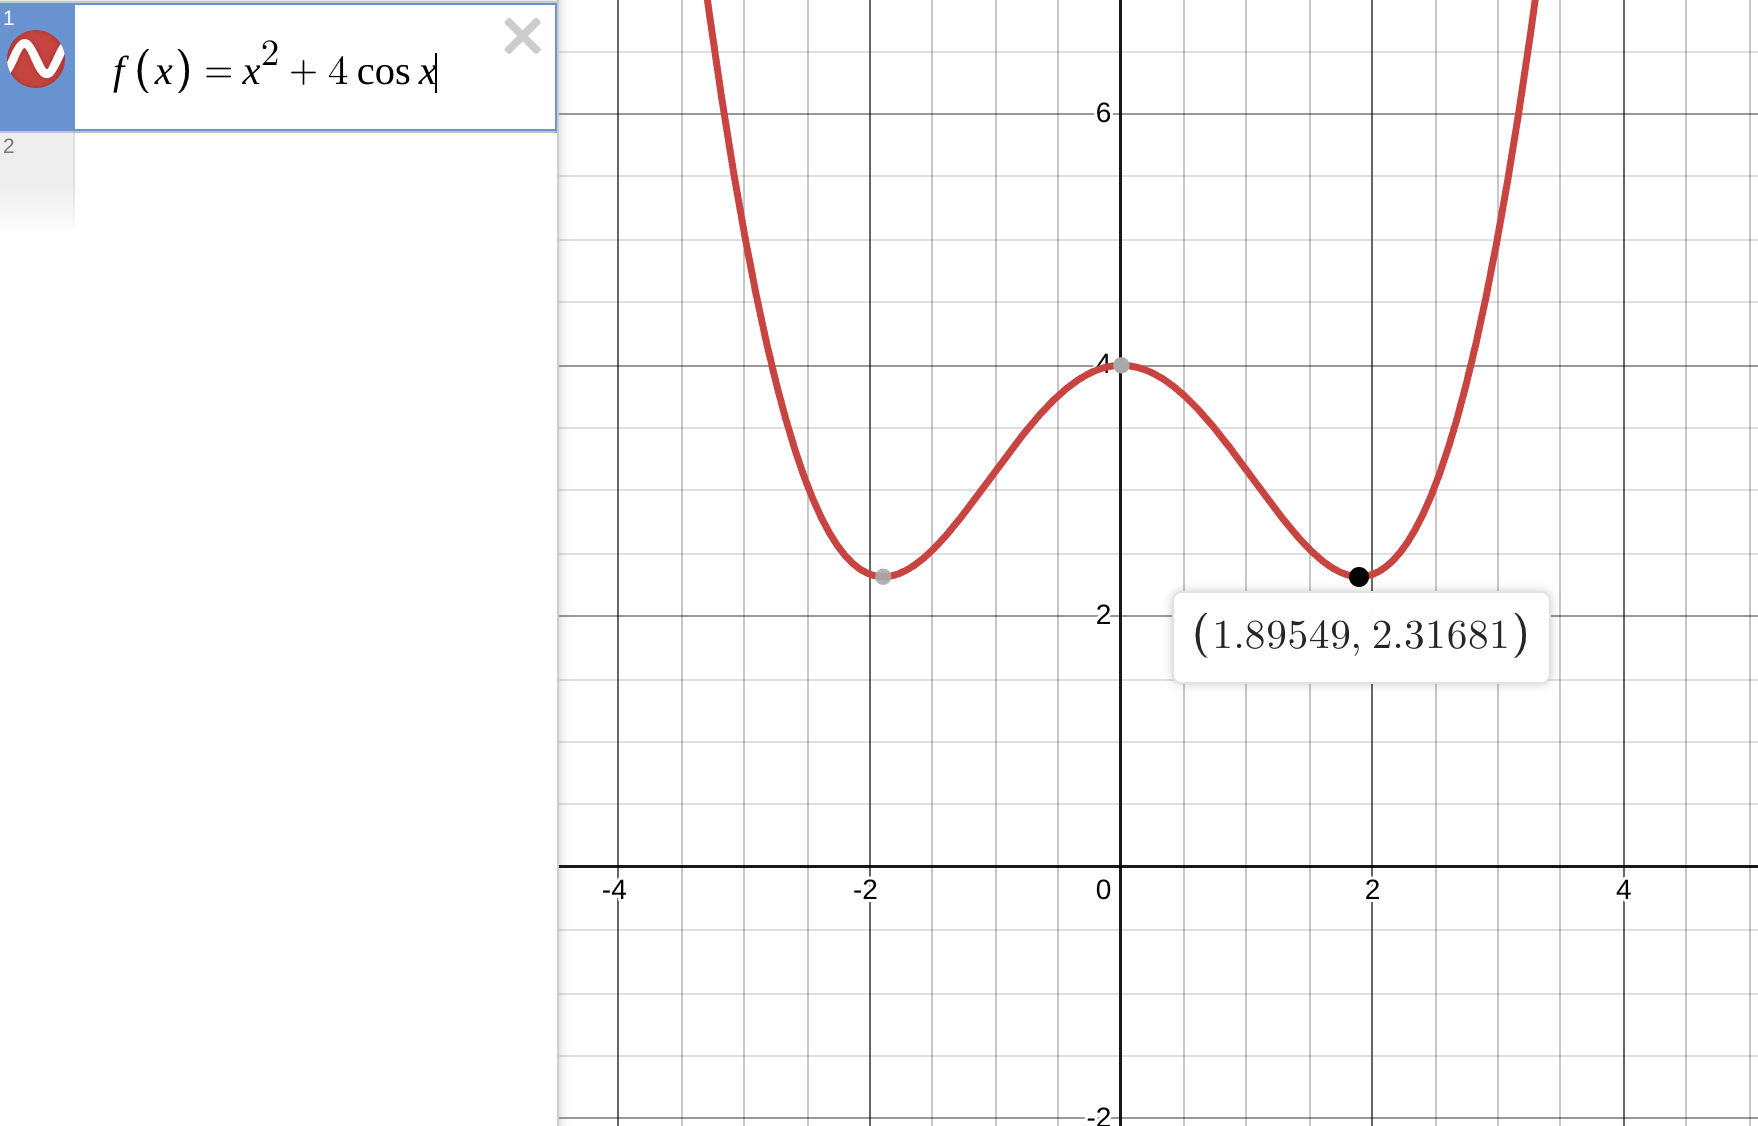
\includegraphics[width=0.8\textwidth]{Images/Q2.png}
\end{figure}

\begin{lstlisting}[language=Python]
import numpy as np

def f(x):
    return x**2 + 4 * np.cos(x)

def f_dash(x):
    return 2 * x - 4 * np.sin(x)

def f_double_dash(x):
    return 2 - 4 * np.cos(x)

x = 1.5 #Initial Guess
iterations = 4

for i in range(iterations):
    x = x - f_dash(x) / f_double_dash(x)
    x = max(1, min(x, 2))
    print(f"Iteration {i + 1}: x = {x}, f(x) = {f(x)}")
\end{lstlisting}

We find that the minimizer of the function is \(\boxed{x = 1.8954942672087132}\) and \(f(x) = 2.316808419788213\).

\clearpage

\begin{question*}[3]
    Find the minimum of \(6e^{-2x} + 2x^2\) by each of the following procedures:
    \begin{enumerate}[label=\alph*.]
        \item Golden section method.
        \item Dichotomous search method.
    \end{enumerate}
\end{question*}

\begin{lstlisting}[language=Python]
import numpy as np

def f(x):
    return 6 * np.exp(-2 * x) + 2 * x**2

def golden_section_search(func, a, b, tol=1e-5):
    gr = (np.sqrt(5) + 1) / 2

    c = b - (b - a) / gr
    d = a + (b - a) / gr

    while abs(b - a) > tol:
        if func(c) < func(d):
            b = d
        else:
            a = c

        c = b - (b - a) / gr
        d = a + (b - a) / gr

    return (b + a) / 2

def dichotomous_search(func, a, b, tol=1e-5, delta=1e-6):
    while abs(b - a) > tol:
        mid = (a + b) / 2
        x1 = mid - delta
        x2 = mid + delta

        if func(x1) < func(x2):
            b = x2
        else:
            a = x1

    return (a + b) / 2

a, b = -10, 10

min_golden = golden_section_search(f, a, b)
min_dichotomous = dichotomous_search(f, a, b)
val_golden = f(min_golden)
val_dichotomous = f(min_dichotomous)
\end{lstlisting}

We get that the minimum value of the function is obtained at $\boxed{x = 0.7162034008722994}$ where the value of the function is $\boxed{2.4582964969114216}$ using the golden section method and $\boxed{x = 0.7162021874434947}$ where the value of the function is $\boxed{2.458296496906626}$ using the dichotomous search method.

\clearpage

\begin{question*}[4]
    Consider the problem to minimize 
    \[
    (3 - x_1)^2 + 7(x_2 - x_1^2)^2.
    \]
    Starting from the point \((0,0)\), solve the problem by the following methods. Do the methods converge to the same point? If not, explain.

    \begin{enumerate}[label=\alph*.]
        \item The cyclic coordinate method.
        \item The method of Hooke and Jeeves.
        \item The method of Rosenbrock.
    \end{enumerate}

\end{question*}

\begin{lstlisting}[language=Python]
import numpy as np
from scipy.optimize import minimize

def f(x):
    x1, x2 = x
    return (3 - x1)**2 + 7 * (x2 - x1**2)**2

def gradient(x):
    x1, x2 = x
    df_dx1 = -2 * (3 - x1) - 28 * x1 * (x2 - x1**2)
    df_dx2 = 14 * (x2 - x1**2)
    return np.array([df_dx1, df_dx2])

initial_point = np.array([0, 0])

def cyclic_coordinate_method(func, x0, tol=1e-6, max_iter=1000, step_size=0.1):
    x = x0.copy()
    n = len(x)
    
    for _ in range(max_iter):
        old_x = x.copy()
        for i in range(n):
            while True:
                f_current = func(x)
                
                x[i] += step_size
                f_new = func(x)
                
                if f_new < f_current:
                    continue
                
                x[i] -= 2 * step_size
                f_new = func(x)
                
                if f_new < f_current:
                    continue
                
                x[i] += step_size
                break
        
        if np.linalg.norm(x - old_x) < tol:
            break
    
    return x

def hooke_jeeves(func, x0, step_size=0.5, alpha=2.0, tol=1e-6, max_iter=1000):
    x = x0.copy()
    n = len(x)
    
    def explore(xb, step):
        x_new = xb.copy()
        for i in range(n):
            f_before = func(x_new)
            x_new[i] += step
            if func(x_new) >= f_before:
                x_new[i] -= 2 * step
                if func(x_new) >= f_before:
                    x_new[i] += step
        return x_new
    
    for _ in range(max_iter):
        xb = x.copy()
        xe = explore(x, step_size)
        
        if np.linalg.norm(xe - x) < tol:
            break
        
        x = xe if func(xe) < func(x) else x
        
        xb_new = x + alpha * (x - xb)
        if func(xb_new) < func(x):
            x = xb_new
        else:
            step_size *= 0.5
    
    return x
    
def rosenbrock_method(func, grad, x0, learning_rate=0.001, tol=1e-6, max_iter=10000):
    x = x0.copy()
    for _ in range(max_iter):
        grad_val = grad(x)
        x_new = x - learning_rate * grad_val
        
        if np.linalg.norm(x_new - x) < tol:
            break
        
        x = x_new
    return x

cyclic_result = cyclic_coordinate_method(f, initial_point)
hooke_jeeves_result = hooke_jeeves(f, initial_point)
rosenbrock_result = rosenbrock_method(f, gradient, initial_point)
\end{lstlisting}

The differences in the results from the three optimization methods can be attributed to their underlying mechanisms and how they explore the search space.
\subsubsection*{1. Cyclic Coordinate Method}
\begin{itemize}
    \item \textbf{Result:} \((0, 0)\)
    \item \textbf{Explanation:} This method optimizes one variable at a time while keeping others fixed. When optimizing \(x_1\) while fixing \(x_2\) at 0, it finds that \(x_1 = 3\) minimizes the function. However, when subsequently optimizing \(x_2\) with \(x_1\) fixed, no improvement is found, leading to the convergence at \((0, 0)\).
\end{itemize}

\subsubsection*{2. Hooke and Jeeves Method}
\begin{itemize}
    \item \textbf{Result:} \((0, 0)\)
    \item \textbf{Explanation:} \textls[-30]{This method explores the search space in a pattern-search manner. If it does not find better points in the vicinity of \((0, 0)\), it may converge there. Insufficient exploration or small step sizes could contribute to this outcome.}
\end{itemize}

\subsubsection*{3. Rosenbrock Method (Gradient Descent)}
\begin{itemize}
    \item \textbf{Result:} \((2.4128, 5.8051)\)
    \item \textbf{Explanation:} Utilizing the gradient of the function, this method finds the minima. It finds a minima at \((2.4128, 5.8051)\), indicating that it can escape the local minimum found by the other methods.
\end{itemize}


\begin{question*}[5]
Show how Newton's method can be used to find a point where the value of a continuously differentiable function is equal to zero. Illustrate the method for \( f(x) = 2x^2 - 5x \) starting from \( x = 5 \).
\end{question*}

Newton's method is an iterative numerical technique used to approximate the roots (or zeros) of a real-valued function. The method relies on the idea of linear approximation and is particularly effective for continuously differentiable functions.

Given a continuously differentiable function \( f: \mathbb{R} \to \mathbb{R} \), we seek a point \( x \) such that:

\[
    f(x) = 0.
\]

The iteration formula for Newton's method is given by:

\[
    x_{n+1} = x_n - \dfrac{f(x_n)}{f'(x_n)}
\]

We start with an initial guess \( x_0 \) and iterate until the function value is within a specified tolerance level.


\begin{lstlisting}[language=Python]
import numpy

def f(x):
    return 2 * x**2 - 5 * x

def f_dash(x):
    return 4 * x - 5

def newton_method(initial_guess, tolerance=1e-7, max_iterations=1000):
    x = initial_guess
    for iteration in range(max_iterations):
        fx = f(x)
        derivative = f_dash(x)
        
        if derivative == 0:
            return None
        
        x = x - fx / derivative
        
        print(f"Iteration {iteration + 1}: x = {x}, f(x) = {f(x)}")
        
        if abs(f(x)) < tolerance:
            return x
    
    return None

initial_guess = 5
newton_method(initial_guess)

\end{lstlisting}

\clearpage

\begin{question*}[6]
Consider the following problem:

\[
    \text{minimize } f(t) = e^{-t} + e^t
\]

in the interval \([-1, 1]\).

Find the optimal value within a tolerance band less than \(0.15\) using:

\begin{itemize}
    \item[(a)] Golden section method
    \item[(b)] Fibonacci method
    \item[(c)] Armijo line search
\end{itemize}

Do you get the same point? If not, explain.
\end{question*}

\begin{lstlisting}[language=Python]
import numpy as np

def f(t):
    return np.exp(-t) + np.exp(t)

def golden_section_method(a, b, tol=0.15, max_iter=100):
    phi = (1 + np.sqrt(5)) / 2
    iter_count = 0
    while (b - a) > tol and iter_count < max_iter:
        c = b - (b - a) / phi
        d = a + (b - a) / phi
        if f(c) < f(d):
            b = d
        else:
            a = c
        iter_count += 1
    return (a + b) / 2

def fibonacci_method(a, b, tol=0.15, max_iter=100):
    n = 1
    while (b - a) > tol and n < max_iter:
        n += 1

    fib = [0, 1]
    for i in range(2, n + 1):
        fib.append(fib[-1] + fib[-2])

    for i in range(1, n):
        r1 = a + (fib[n - i - 1] / fib[n]) * (b - a)
        r2 = a + (fib[n - i] / fib[n]) * (b - a)

        if f(r1) < f(r2):
            b = r2
        else:
            a = r1

    return (a + b) / 2

def armijo_line_search(t0, alpha=0.1, beta=0.5, tol=0.15, max_iter=100):
    t = t0
    iter_count = 0
    while iter_count < max_iter:
        gradient = -np.exp(-t) + np.exp(t)  # f'(t)
        t_new = t - alpha * gradient
        if f(t_new) <= f(t) + beta * alpha * gradient:
            t = t_new
        if abs(f(t_new) - f(t)) < tol:
            break
        iter_count += 1
    return t

a, b = -1, 1
tol = 0.15
max_iter = 10000

golden_result = golden_section_method(a, b, tol, max_iter)
fibonacci_result = fibonacci_method(a, b, tol, max_iter)
armijo_result = armijo_line_search(0, tol=tol, max_iter=max_iter)
\end{lstlisting}

The three outputs obtained from the optimization methods are as follows:
\begin{itemize}
    \item Golden Section Method: \( t \approx 7.63 \times 10^{-17} \)
    \item Fibonacci Method: \( t \approx -0.0802 \)
    \item Armijo Line Search: \( t = 0.0 \)
\end{itemize}

The differences in the outputs can be attributed to several factors:

The function \( f(t) = e^{-t} + e^{t} \) is convex over the interval \([-1, 1]\). However, due to its exponential growth, small variations in the methods can lead to different evaluations around the minimum point.

\begin{itemize}
   \item \textbf{Golden Section Method} and \textbf{Fibonacci Method}: These interval-based methods rely on point evaluations within a specified interval, narrowing the search space based on comparisons of function values. The final outcome can differ based on the initial interval.
   \item \textbf{Armijo Line Search}: This gradient-based approach starts from an initial point and iteratively updates based on the gradient's direction. Sensitivity to step size choices can lead to different outcomes, particularly in non-strictly convex functions.
\end{itemize}

Each method's convergence criteria, defined by tolerance and maximum iterations, can lead to different stopping points. A higher tolerance or reaching maximum iterations before convergence can cause varied results.

\begin{question*}[7]
Consider the following problem:

\[
\text{maximize } f(x) = (\sin(x))^6 \tan(1 - x) e^{30x}
\]

in the interval \([0, 1]\). Find the optimal point within a tolerance band less than \(0.15\) using:

\begin{itemize}
    \item[(a)] Golden ratio method
    \item[(b)] Quadratic interpolation method
    \item[(c)] Goldstein line search
\end{itemize}
\end{question*}

\begin{lstlisting}[language=Python]
import numpy as np

def f(x):
    return (np.sin(x))**6 * np.tan(1 - x) * np.exp(30 * x)

def golden_ratio_method(a, b, tol, max_iter):
    phi = (-1 + np.sqrt(5)) / 2
    
    x1 = b - phi * (b - a)
    x2 = a + phi * (b - a)
    
    f1 = f(x1)
    f2 = f(x2)

    iterations = 0
    while (b - a) > tol and iterations < max_iter:
        if f1 < f2:
            b = x2
            x2 = x1
            f2 = f1
            x1 = b - phi * (b - a)
            f1 = f(x1)
        else:
            a = x1
            x1 = x2
            f1 = f2
            x2 = a + phi * (b - a)
            f2 = f(x2)
        iterations += 1

    return (a + b) / 2, f((a + b) / 2)

def quadratic_interpolation_method(a, b, tol, max_iter):
    x0 = a
    x1 = (a + b) / 2
    x2 = b

    iterations = 0
    while (b - a) > tol and iterations < max_iter:
        f0, f1, f2 = f(x0), f(x1), f(x2)
        denominator = (x0 - x1) * (x0 - x2) * (x1 - x2)
        if denominator == 0:
            break  # Avoid division by zero
        x_new = (f0 * (x1 - x2) + f1 * (x2 - x0) + f2 * (x0 - x1)) / (f0 * (x1 - x2) + f1 * (x2 - x0) + f2 * (x0 - x1))
        
        if x_new < a or x_new > b:
            break  # Ensure new point is within bounds

        if f(x_new) > f(x1):
            x0, x1, x2 = x1, x_new, x2
        else:
            x0, x1, x2 = x0, x1, x_new

        iterations += 1

    return (x0 + x1 + x2) / 3, f((x0 + x1 + x2) / 3)

def f_prime(x):  # Numerical derivative using central difference (because im too lazy to calculate the actual derivative and I don't want to use the scipy function)
    h = 1e-5
    return (f(x + h) - f(x - h)) / (2 * h)

def goldstein_line_search(x0, direction, alpha=0.1, beta=0.9, max_iter=100):
    x1 = x0 + direction
    iterations = 0

    while (f(x1) > f(x0) + alpha * (x1 - x0) * f_prime(x0) and f(x1) < f(x0) + beta * (x1 - x0) * f_prime(x0)) and iterations < max_iter:
        x1 -= direction
        iterations += 1
    
    return x1, f(x1)

a, b = 0, 1
tolerance = 0.15
max_iterations = 1000
optimum_golden = golden_ratio_method(a, b, tolerance, max_iterations)
optimum_quad = quadratic_interpolation_method(a, b, tolerance, max_iterations)
x0 = 0.5  # starting point
direction = 0.1  # arbitrary small step
optimum_goldstein = goldstein_line_search(x0, direction, max_iter=max_iterations)
\end{lstlisting}

We get that the optimal point obtained by the three optimization methods are as follows:

\begin{itemize}
    \item Golden Ratio Method: $x = 0.6909830056250525 , f(x) = 21521325.939824104$
    \item Quadratic Interpolation Method: $x = 0.5 , f(x) = 21685.897332525412$
    \item Goldstein Line Search: $x = 0.6 , f(x) = 899642.4669646018$
\end{itemize}


\begin{question*}[8]
Consider the function \( f: \mathbb{R}^2 \to \mathbb{R} \),

\[
f(x_1, x_2) = 100(x_2 - x_1^2)^2 + (1 - x_1)^2.
\]

Write a program in MATLAB/C/Python for the steepest descent algorithm using the backtracking line search to find the extrema. Set the initial step-length \( \alpha_0 = 1 \) and print the step length used by each method in each iteration. Update the step size \( \alpha_k \) at every iteration to satisfy the Goldstein condition. The initial point is given as \( x_0 = (1.2, 1.2)^\mathsf{T} \).
\end{question*}

\begin{lstlisting}[language=Python]
import numpy as np

def f(x):
    x1, x2 = x
    return 100 * (x2 - x1**2)**2 + (1 - x1)**2

def grad_f(x):
    x1, x2 = x
    df_dx1 = -400 * x1 * (x2 - x1**2) - 2 * (1 - x1)
    df_dx2 = 200 * (x2 - x1**2)
    return np.array([df_dx1, df_dx2])

def backtracking_line_search(x, p, alpha=1, rho=0.9, c=1e-4):
    while f(x + alpha * p) > f(x) + c * alpha * np.dot(grad_f(x), p):
        alpha *= rho
    return alpha

def steepest_descent(x0, tol=1e-4, max_iter=1000):
    x = x0
    alpha = 1  # Initial step length
    iterations = []

    for i in range(max_iter):
        gradient = grad_f(x)
        if np.linalg.norm(gradient) < tol:
            break

        p = -gradient
        alpha = backtracking_line_search(x, p) 
        x = x + alpha * p 

        iterations.append((i + 1, x, alpha)) 

    return x, iterations

x0 = np.array([1.2, 1.2])
result, iterations = steepest_descent(x0)

print(f"Optimal point: {result}")
print("Iterations (index, x, step length):")
for iteration in iterations:
    print(iteration)
\end{lstlisting}


\begin{question*}[9]
Consider the following problem:

\[
\text{minimize } f(x_1, x_2) = 32x_1^2 + 12x_2^2 - x_1 x_2 - 2x_1
\]

with initial point \( (-2, 4)^\mathsf{T} \).

Solve the problem by:

\begin{itemize}
    \item[(a)] Steepest descent method
    \item[(b)] Newton's method
\end{itemize}
\end{question*}

\begin{lstlisting}[language=Python]
import numpy as np

def f(x):
    return 32 * x[0]**2 + 12 * x[1]**2 - x[0] * x[1] - 2 * x[0]

def gradient(x):
    dfdx1 = 64 * x[0] - x[1] - 2
    dfdx2 = 24 * x[1] - x[0]
    return np.array([dfdx1, dfdx2])

def hessian(x):
    d2fdx1dx1 = 64
    d2fdx1dx2 = -1
    d2fdx2dx2 = 24
    return np.array([[d2fdx1dx1, d2fdx1dx2], [d2fdx1dx2, d2fdx2dx2]])

def steepest_descent(initial_point, learning_rate=0.01, tolerance=1e-6, max_iter=1000):
    x = np.array(initial_point)
    for i in range(max_iter):
        grad = gradient(x)
        x_new = x - learning_rate * grad
        if np.linalg.norm(x_new - x) < tolerance:
            # print(f"Converged in {i} iterations.")
            break
        x = x_new
    return x

def newtons_method(initial_point, tolerance=1e-6, max_iter=1000):
    x = np.array(initial_point)
    for _ in range(max_iter):
        grad = gradient(x)
        hess = hessian(x)
        x_new = x - np.linalg.inv(hess).dot(grad)
        if np.linalg.norm(x_new - x) < tolerance:
            break
        x = x_new
    return x

initial_point = (-2, 4)
optimal_sd = steepest_descent(initial_point)
optimal_nm = newtons_method(initial_point)
\end{lstlisting}

\clearpage

\begin{question*}[10]
Consider the problem to minimize 

\[
f(x) = 3x - 2x^2 + x^3 + 2x^4
\]

subject to \( x \geq 0 \).

\begin{enumerate}[label=\alph*.]
    \item Write a necessary condition for a minimum. Can you make use of this condition to find the global minimum?
    \item Is the function strictly quasiconvex over the region \( \{ x : x \geq 0 \} \)? Apply the Fibonacci search method to find the minimum.
    \item Apply both the bisection search method and Newton's method to the above problem, starting from \( x_1 = 6 \).
\end{enumerate}
\end{question*}

\subsection*{Part (a)}

1. \textbf{Necessary Condition}: To find the critical points, we first compute the derivative of \( f(x) \) and set it equal to zero.

   \[
   f'(x) = 3 - 4x + 3x^2 + 8x^3
   \]
   
   Setting \( f'(x) = 0 \) gives the equation:
   
   \[
   3 - 4x + 3x^2 + 8x^3 = 0
   \]
   
   Solving this equation for \( x \) gives us the critical points, which are candidates for minima or maxima.

2. \textbf{Second Derivative Test}: To determine if these critical points are minima, we calculate the second derivative \( f''(x) \):

   \[
   f''(x) = -4 + 6x + 24x^2
   \]

   We evaluate \( f''(x) \) at each critical point. If \( f''(x) > 0 \) at a point, it indicates a local minimum. To determine if any of these points is a global minimum, we analyze \( f'(x) \) and \( f''(x) \) over the feasible region \( x \geq 0 \).

\subsection*{Part (b)}

A function is \underline{strictly quasiconvex} if every set \( \{ x : f(x) \leq \alpha \} \) is a strictly convex set. To check this:

1. \textbf{Derivative Behavior}: We analyze the behavior of \( f(x) \) on \( x \geq 0 \). If \( f(x) \) does not exhibit multiple local minima over this interval, it may be quasiconvex. However, strict quasiconvexity requires further verification of each of the individual sets.

2. \textbf{Monotonicity}: If \( f(x) \) strictly decreases and then strictly increases around a minimum, it could be considered quasiconvex.

We see that both the first and second derivatives of \( f(x) \) are continuous and differentiable over \( x \geq 0 \). The function is \boxed{\text{not strictly quasiconvex}}, as it exhibits multiple local minima over the region.

\subsubsection*{Fibonacci Search Method}
The \textbf{Fibonacci search method} is a bracketing method for finding the minimum of a function:

- Define an initial interval \( [a, b] \) (e.g., \( a = 0 \) and \( b = 6 \) if this captures the region around the critical points). \\
- At each step, evaluate \( f(x) \) at points determined by Fibonacci ratios and reduce the interval of uncertainty. \\
- Repeat until the interval is sufficiently small (smaller than the tolerance levels).

\subsection*{Part (c)}

We apply the following search methods to find the minimum of \( f(x) \) over \( x \geq 0 \):

\subsubsection*{1. Bisection Search Method}
The \textbf{bisection search method} proceeds as follows:

- Start with an interval \( [a, b] \) (e.g., \( [0, 6] \)). \\
- At each iteration, calculate the midpoint \( x = \frac{a + b}{2} \) and evaluate \( f'(x) \). \\
- Adjust \( a \) or \( b \) based on where the derivative changes sign, narrowing down the interval. \\
- Continue until the interval is sufficiently small (smaller than the tolerance levels).

\subsubsection*{2. Newton's Method}
\textbf{Newton’s method} is an iterative method that updates \( x \) using the formula:

\[
x_{n+1} = x_n - \frac{f'(x_n)}{f''(x_n)}
\]

- Start with an initial guess, say \( x_1 = 6 \). \\
- Iterate until \( f'(x) \approx 0 \), indicating a minimum.

\begin{lstlisting}[language=Python]
import numpy as np

def f(x):
    return 3*x - 2*x**2 + x**3 + 2*x**4

def f_dash(x):
    return 3 - 4*x + 3*x**2 + 8*x**3

def f_double_dash(x):
    return -4 + 6*x + 24*x**2

def bisection_search(a, b, tol=1e-5, max_iter=100):
    if a < 0:
        a = 0
    if b < 0:
        return None
    
    iter_count = 0
    while (b - a) > tol and iter_count < max_iter:
        mid = (a + b) / 2
        if f_dash(mid) == 0:
            return mid
        elif f_dash(mid) * f_dash(a) < 0:
            b = mid
        else:
            a = mid
        iter_count += 1
        
    return (a + b) / 2 if iter_count < max_iter else None

def newton_method(x0, tol=1e-5, max_iter=100):
    x = max(x0, 0)
    iter_count = 0
    
    while iter_count < max_iter:
        x_new = x - f_dash(x) / f_double_dash(x)
        x_new = max(x_new, 0)  # Ensure x_new is non-negative
        if abs(x_new - x) < tol:
            return x_new
        x = x_new
        iter_count += 1
    
    return None 

def fibonacci_search(a, b, tol=1e-5, max_iter=100):
    if a < 0:
        a = 0
    if b < 0: 
        return None 

    fib = [0, 1]
    while len(fib) < max_iter + 2:
        fib.append(fib[-1] + fib[-2])
    
    n = len(fib) - 2
    if n < 2:
        return None 

    x1 = a + fib[n - 2] / fib[n] * (b - a)
    x2 = a + fib[n - 1] / fib[n] * (b - a)

    iter_count = 0
    while iter_count < max_iter:
        if f(x1) < f(x2):
            b = x2
        else:
            a = x1
        
        if abs(b - a) <= tol:
            break

        iter_count += 1

        if n - iter_count >= 2:
            x1 = a + fib[n - iter_count - 2] / fib[n - iter_count] * (b - a)
            x2 = a + fib[n - iter_count - 1] / fib[n - iter_count] * (b - a)
        else:
            break  

    return (a + b) / 2 if iter_count < max_iter else None

x_start = 6
tol = 1e-5
a, b = 0, x_start 

bisection_result = bisection_search(a, b)
newton_result = newton_method(x_start)
fibonacci_result = fibonacci_search(a, b)
\end{lstlisting}


\end{document}